\documentclass[border=10pt]{standalone}
\usepackage{tikz}
\usetikzlibrary{positioning, arrows.meta, calc, fit, decorations.pathreplacing}
\usepackage{amsmath,amssymb}

\begin{document}

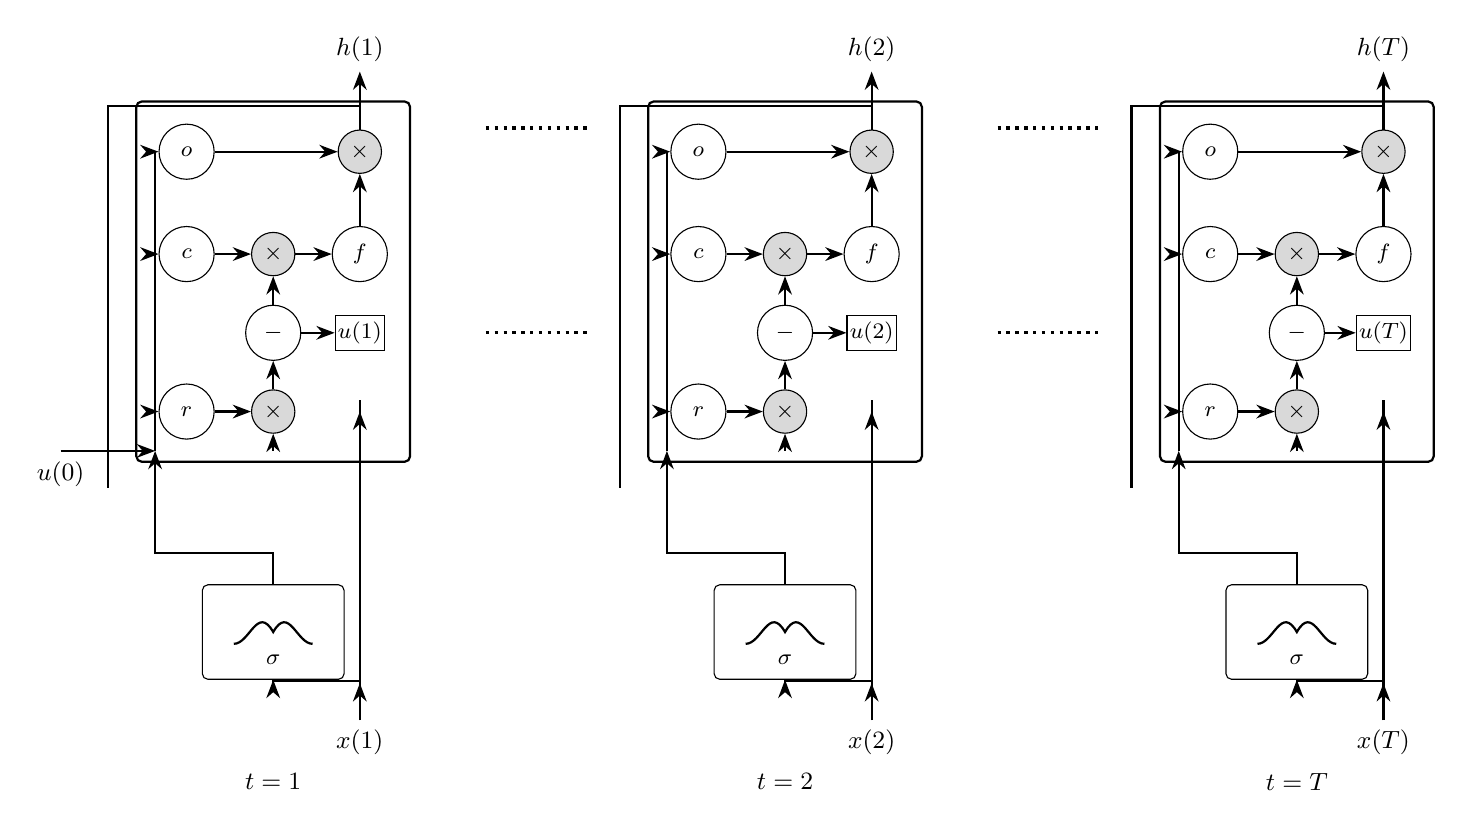
\begin{tikzpicture}[
    >=Stealth,
    node distance=0.6cm,
    % Gate circle style (white fill)
    gate/.style={circle, draw, minimum size=0.7cm, inner sep=0pt, font=\footnotesize},
    % Operation circle (gray fill)
    op/.style={circle, draw, fill=gray!30, minimum size=0.55cm, inner sep=0pt, font=\footnotesize},
    % Box style for u(t) / subtraction
    boxnode/.style={rectangle, draw, minimum width=0.6cm, minimum height=0.45cm, inner sep=1pt, font=\footnotesize},
    % The main LSTM cell bounding box
    cellbox/.style={draw, rounded corners=2pt, inner sep=8pt, thick},
    % Fuzzy block
    fuzzybox/.style={draw, rounded corners=2pt, inner sep=5pt, minimum width=1.8cm, minimum height=1.2cm},
    % Arrow style
    arr/.style={->, thick},
    every node/.style={font=\small},
]

% ============================================================
% Helper macro: draw one LSTM-SNP cell with fuzzy input
% Arguments: #1=x-offset, #2=time label (1,2,T)
% ============================================================
\newcommand{\drawcell}[2]{
    \begin{scope}[xshift=#1 cm]

    % --- FUZZY FEATURE AUGMENTATION BLOCK (below the cell) ---
    \node[fuzzybox] (fuzzy#2) at (1.5, -2.8) {};
    
    % Gaussian curve inside fuzzy box
    \draw[thick] ([xshift=-0.5cm, yshift=-0.15cm]fuzzy#2.center) 
        .. controls ([xshift=-0.3cm, yshift=-0.15cm]fuzzy#2.center) 
        and ([xshift=-0.2cm, yshift=0.35cm]fuzzy#2.center) 
        .. (fuzzy#2.center)
        .. controls ([xshift=0.2cm, yshift=0.35cm]fuzzy#2.center) 
        and ([xshift=0.3cm, yshift=-0.15cm]fuzzy#2.center) 
        .. ([xshift=0.5cm, yshift=-0.15cm]fuzzy#2.center);
    
    \node[font=\footnotesize] at ([yshift=-0.35cm]fuzzy#2.center) {$\sigma$};
    
    % --- MAIN LSTM-SNP CELL ---
    % Gates (from bottom to top): r, -, c, o
    % r gate
    \node[gate] (r#2) at (0.4, 0) {$r$};
    % multiply after r
    \node[op] (rmul#2) at (1.5, 0) {$\times$};
    
    % subtraction node
    \node[gate] (sub#2) at (1.5, 1.0) {$-$};
    % u(t) box
    \node[boxnode] (u#2) at (2.6, 1.0) {$u(#2)$};
    
    % c gate
    \node[gate] (c#2) at (0.4, 2.0) {$c$};
    % multiply after c
    \node[op] (cmul#2) at (1.5, 2.0) {$\times$};
    % f gate
    \node[gate] (f#2) at (2.6, 2.0) {$f$};
    
    % o gate
    \node[gate] (o#2) at (0.4, 3.3) {$o$};
    % multiply after o
    \node[op] (omul#2) at (2.6, 3.3) {$\times$};
    
    % --- Connections inside the cell ---
    % r -> rmul
    \draw[arr] (r#2) -- (rmul#2);
    % rmul -> sub
    \draw[arr] (rmul#2) -- (sub#2);
    % sub -> u
    \draw[arr] (sub#2) -- (u#2);
    % sub -> cmul (upward)
    \draw[arr] (sub#2) -- (cmul#2);
    % c -> cmul
    \draw[arr] (c#2) -- (cmul#2);
    % cmul -> f (right)
    \draw[arr] (cmul#2) -- (f#2);
    
    % f -> omul (upward)
    \draw[arr] (f#2) -- (omul#2);
    % o -> omul (connect via right path)
    \draw[arr] (o#2) -- ++(0.5, 0) |- (omul#2);
    
    % --- Bounding box ---
    \node[cellbox, fit=(r#2)(o#2)(omul#2)(f#2)(u#2), 
          label={[font=\small]below right:}] (box#2) {};
    
    % --- Input x(t) arrow from bottom ---
    \node[font=\small] (xlabel#2) at (2.6, -4.2) {$x(#2)$};
    \draw[arr] (xlabel#2) -- (2.6, -3.5) -- (2.6, -3.45);
    
    % Split: one path to fuzzy block, one path into cell
    % x -> fuzzy block
    \draw[arr] (xlabel#2.north) -- ++(0, 0.5) -| (fuzzy#2.south);
    
    % fuzzy block -> into cell (bottom-left)
    \draw[arr] (fuzzy#2.north) -- ++(0, 0.4) -| (0.0, -0.5);
    
    % Left input line going up to all gates
    \draw[thick] (0.0, -0.5) -- (0.0, 3.3);
    \draw[arr] (0.0, 0) -- (r#2.west);
    \draw[arr] (0.0, 2.0) -- (c#2.west);
    \draw[arr] (0.0, 3.3) -- (o#2.west);
    
    % x(t) direct path also feeds right side (into rmul, f)
    \draw[thick] (2.6, -3.45) -- (2.6, -0.5);
    \draw[thick] (2.6, -0.5) -- (2.6, 0);
    \draw[arr] (2.6, 0) -- (rmul#2.east -| 2.6, 0) -- ++(0, 0);
    
    % Right input feeds rmul from below and f from below
    \draw[thick] (2.6, -0.5) -- (2.6, 0);
    \draw[arr] (1.5, -0.5) -- (rmul#2);
    
    % --- Output h(t) from top ---
    \node[font=\small] (hlabel#2) at (2.6, 4.6) {$h(#2)$};
    \draw[arr] (omul#2) -- (hlabel#2);
    
    % --- Recurrent connection (left side, from top going around) ---
    % h -> feeds back left
    \draw[thick] (omul#2.north) -- ++(0, 0.3) -- ++(-3.2, 0) -- ++(0, -4.85);
    
    % --- u(t-1) feeding into the left (previous state) ---
    
    % --- Time step label ---
    \node[font=\small] at (1.5, -4.7) {$t=#2$};
    
    \end{scope}
}

% ============================================================
% Draw three cells
% ============================================================

% Cell t=1
\drawcell{0}{1}

% Cell t=2
\drawcell{6.5}{2}

% Dotted connection between cell 1 and cell 2
\draw[dotted, very thick] (4.2, 1.0) -- (5.5, 1.0);
\draw[dotted, very thick] (4.2, 3.6) -- (5.5, 3.6);

% Cell t=T
\drawcell{13}{T}

% Dotted connection between cell 2 and cell T
\draw[dotted, very thick] (10.7, 1.0) -- (12.0, 1.0);
\draw[dotted, very thick] (10.7, 3.6) -- (12.0, 3.6);

% --- u(0) label on the far left ---
\node[font=\small] at (-1.2, -0.8) {$u(0)$};
\draw[arr] (-1.2, -0.5) -- (-0.5, -0.5) -- (0.0, -0.5);

\end{tikzpicture}

\end{document}
